\section{Test setup}
The purpose of this section is to present the demo assembly and its'  individual parts. Furthermore this section introduces the test setup consisting of a Adept robot and a conveyor belt, and will analyse the physical work space and which modifications are necessary.  
%The purpose of this section is to present and describe the test setup consisting of a Adept robot and a conveyor belt. Likewise this section will introduce the object which the robot will perform the pick and place operation with. The object is an assembly and the description will consist of a presentation of the individual parts geometry and material. 

\subsection{The Assembly}
The demo assembly is made for production line tests and is shown on figure \ref{fig_assembly} and the assembly order is shown as a exploded view on figure \ref{fig_exploded}. 
\begin{figure}[htbp!]
\centering
\begin{subfigure}[t]{0.45\textwidth}
\centering
\includegraphics[width=\textwidth]{prob_ana_emne}
\caption{The assembly}
\label{fig_assembly}  
\end{subfigure}~~
\begin{subfigure}[t]{0.45\textwidth}
\centering
\includegraphics[width=\textwidth]{prob_ana_emne_exploded}
\caption{Exploded view showing the assembly order of the assembly}
\label{fig_exploded}  
\end{subfigure}
\caption{}
\end{figure}\newline
\noindent The assembly consist of a housing, the PCB, two fuses which are inserted into a spring socket and a lid, the lid and housing comes in both black and blue. Today Aalborg University uses the demo assembly for their existing smart lab, which is a production line built with interchangeable modules. A picture of this production line is shown on figure \ref{fig_smart_lab}.
\begin{figure}[htbp!]
\centering
\begin{subfigure}[t]{0.45\textwidth}
\includegraphics[width=\textwidth]{smart_lab}
\caption{The smart production lab at Aalborg University}
\label{fig_smart_lab}  
\end{subfigure}~~
\begin{subfigure}[t]{0.5\textwidth}
\includegraphics[width=\textwidth]{assembly_pallet}
\caption{The assembly on the pallet for the smart production}
\label{fig_assembly_pallet}
\end{subfigure}
\caption{}
\end{figure}\newline
The demo assembly is made for this smart production line and it is placed on a pallet, shown on figure \ref{fig_assembly_pallet}, which is then moved around the different modules via a conveyor belt. The smart production line is able to handle mass customisation because each pallet is equipped with a RFID chip. This chip is programmed with all information about what color the housing should be and what manufacturing operations need to be made to the assembly. As it is now, the pallet is moved to a operation station, where the conveyor belt stops until the operation is complete. If the operation is to drill a hole, it is necessary to stop while the hole is being driller. If it instead is to place the lid on the housing with a robot, it is more efficient for the robot to place the lid while the pallet with the housing is passing by. Aalborg University is therefore interested in developing a vision system which makes a robot place a lid with the correct color on the housing. As mentioned, this should be done without the vision system communicating with the smart production line. This means the vision system needs to detect position, orientation and velocity of the housing, such that the robot can match the speed and orient the lid such that it will fit on the housing. The reason for this is, such a solution is fast to implement and flexible since it does not set any requirements for positioning except that the robot should be able to reach the conveyor and there should not be anything the robot can hit within its' work space.


\subsection{The Adept Robot} 
The robot used for this test setup is a Adept Cobra s600 robot, shown on figure \ref{fig_cobra_workspace} and consist of three revolute joints and one prismatic. These joints are indicated on the figure with red lines.
\begin{figure}[htbp!]
\centering
\begin{minipage}[t]{.6\textwidth}
\centering
\vspace{0pt}
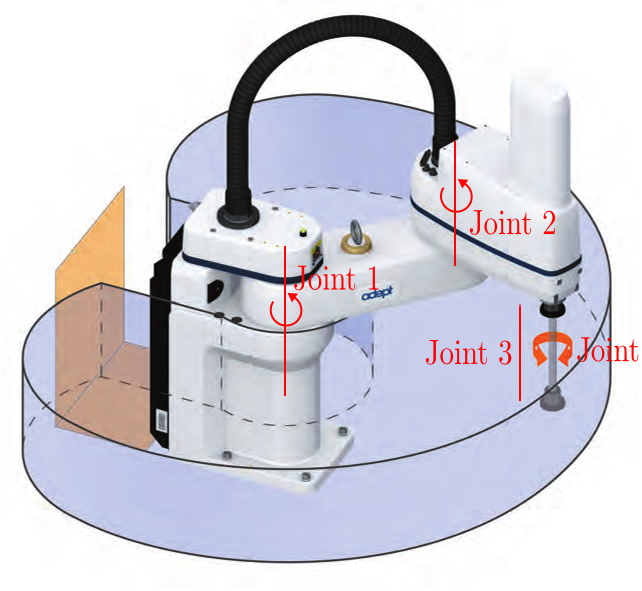
\includegraphics[width=\textwidth]{prob_ana_workspace}
\caption{The available work space for the Cobra s600 \citep[modified]{cobra}}
  \label{fig_cobra_workspace}
\end{minipage}~~
\begin{minipage}[t]{.35\textwidth}
\centering
\vspace{2.85cm}
  \begin{tabular}{c|c}
Joint 1 & $\pm 105^o$\\\hline
Joint 2 & $\pm 150^o$\\\hline
Joint 3 & 210 [mm]\\\hline
Joint 4 & $\pm 360^o$\\\hline
Inner limit & 163 [mm]\\\hline
Outer limit & 600 [mm]\\

  \end{tabular}
  \vspace{2.85cm}
  \captionof{table}{Joint ranges for the Cobra s600 \citep{cobra}}
  \label{tab_joints}
\end{minipage}
\end{figure}\newline
\noindent The work space the robot's end effector is able to reach is determined from the joints, and this available work space is indicated on figure \ref{fig_cobra_workspace} by the blue envelope. The joints' ranges are specified in the datasheet for the Cobra s600, and are summarised in table \ref{tab_joints} along with the inner and outer radius of the work space.\clearpage


 \subsection{Work space} \label{sub_work_space}
With the work space of the Cobra defined, it is now necessary to define the available work space in the test setup. The Cobra is placed inside a cage next to a conveyor belt, shown on figure \ref{fig_pic_setup}. By making a CAD model of the work space, it is possible to better understand possibilities and limitations of it. A plan view of this CAD model is shown on figure \ref{fig_sketch_plan}, where only important features are included.

\begin{figure}[htbp]
\centering
\begin{subfigure}[t]{0.45\textwidth}
\centering
\includegraphics[width=\textwidth]{prob_ana_opstilling}
\caption{Picture of the actual test setup}
\label{fig_pic_setup}


\end{subfigure}~~
\begin{subfigure}[t]{0.45\textwidth}
\centering
\includegraphics[width=\textwidth]{prob_ana_plan}
\caption{Plan view of the work space created from the CAD model, all measurements are in millimetre. The CAD model of the Cobra s600 is available online \citep{cobra}}
\label{fig_sketch_plan}

\end{subfigure}
\caption{}
\end{figure} 
\noindent Inside the cage it is necessary to place two lid buffers, one in with blue and one with black lids, inside the pallet area of the plan view. The desired pick and place operation is then to pick a lid in the correct color and place it on the housing. The housing is place in an arbitrary position and orientation on the conveyor and moving with unknown speed that might change. The control of the conveyor belt is done by a frequency transformer, and is not connected to robot control unit. It is therefore necessary for the robot to match the speed of the conveyor belt, when performing the picking operation. For this test setup to be used for vision servoing of the Cobra, it is necessary to modify it with a camera for visual feedback and setup the communication between the robot control unit and the vision system. Furthermore, it is assumed it is necessary to install lighting to ensure proper visual feedback.
